\begin{frame}
\frametitle{The cost of generality, or forwards-compatibility}
\begin{table}
\begin{center}
\begin{scriptsize}
\begin{tabular}{l|l|l|l|l|l}
\bf RemyCC & \bf Link rates & \bf RTT & \bf Senders & ON/OFF time & Topology \\
\hline
1000x  & 1--1000~Mbps & 150~ms & 2  & 1 sec & Dumbbell\\
100x   & 3.2--320~Mbps & 150~ms & 2 & 1 sec & Dumbbell\\
10x    & 10--100~Mbps & 150~ms & 2 & 1 sec & Dumbbell \\
2x     & 22--44~Mbps & 150~ms & 2 & 1 sec & Dumbbell \\
\end{tabular}
\end{scriptsize}
\caption{Training scenarios for forwards-compatibility experiment}
\label{table:oprange}
\end{center}
\end{table}

\begin{table}
\begin{center}
\begin{scriptsize}
\begin{tabular}{l|l|l|l|l}
\bf Link rates & \bf RTT & \bf Senders & ON/OFF time & Topology \\
\hline
1--1000~Mbps & 150~ms & 2  & 1 sec & Dumbbell\\
\end{tabular}
\end{scriptsize}
\caption{Testing scenarios for forwards-compatibility experiment}
\label{table:oprange}
\end{center}
\end{table}

\end{frame}

\begin{frame}
\frametitle{The cost of generality, or forwards-compatibility}
\begin{centering}

\noindent \only<1>{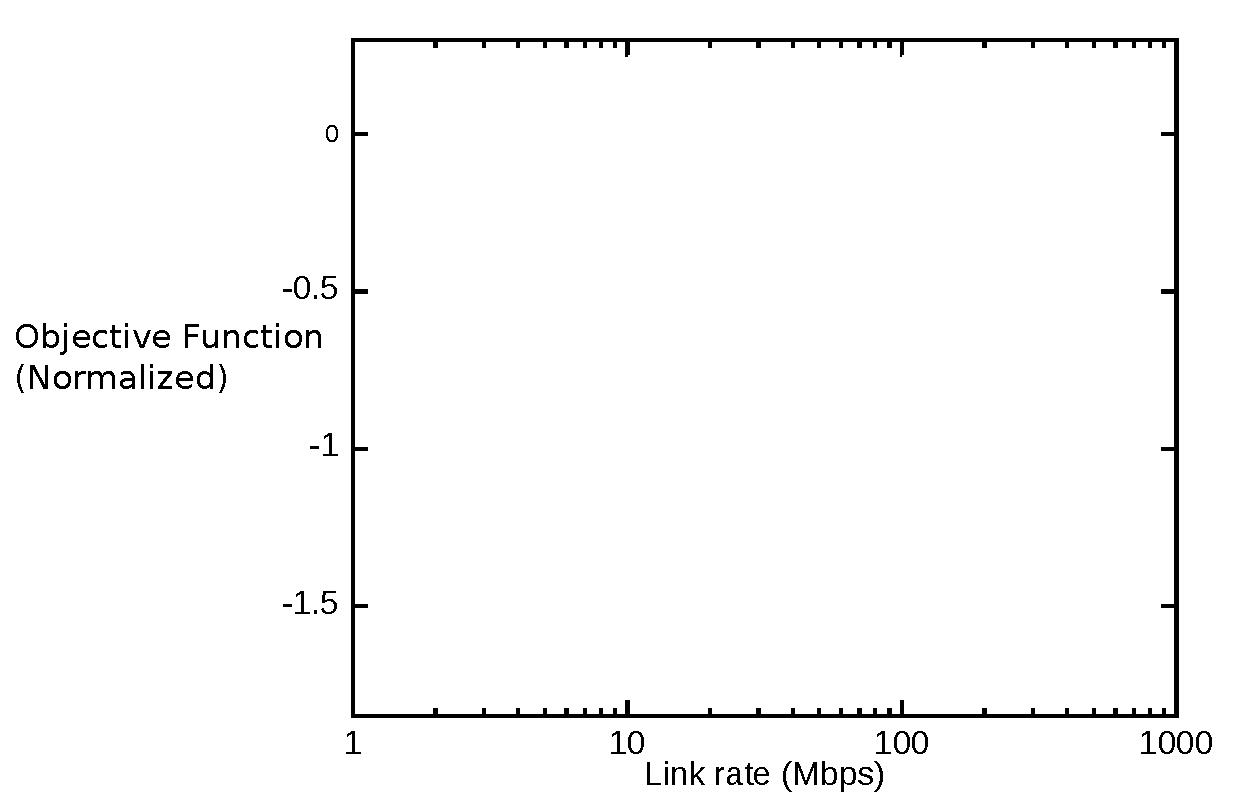
\includegraphics[width=3.1 in]{oprange-base.pdf}}\only<2>{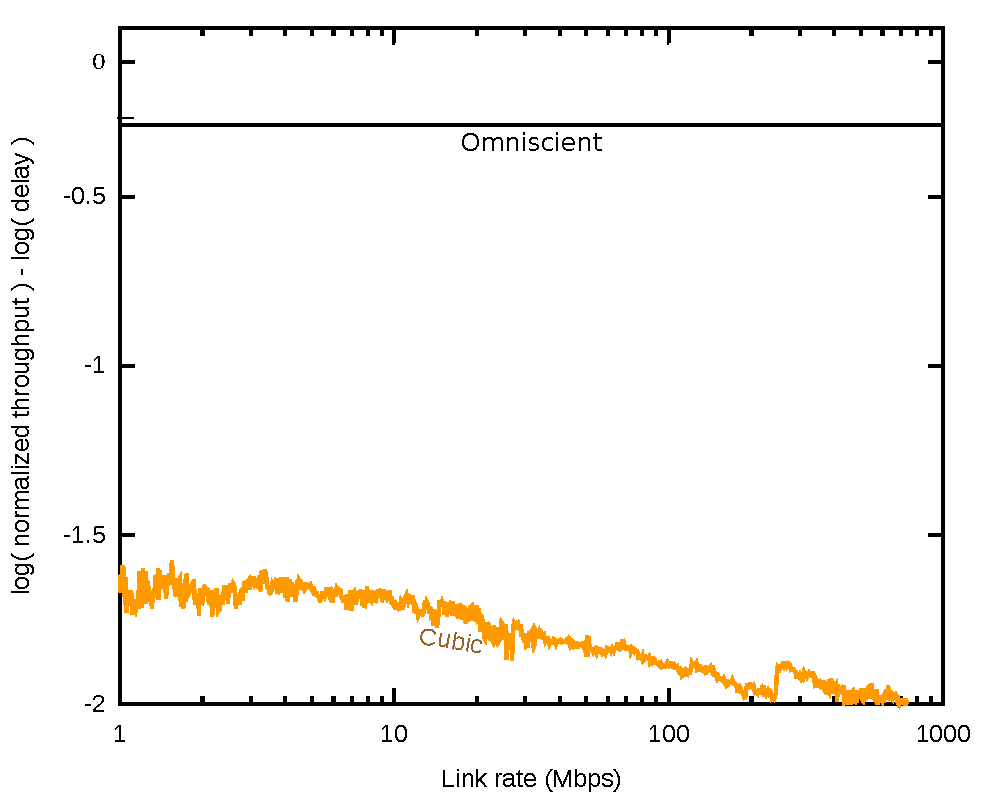
\includegraphics[width=3.1 in]{oprange-cubic.pdf}}\only<3>{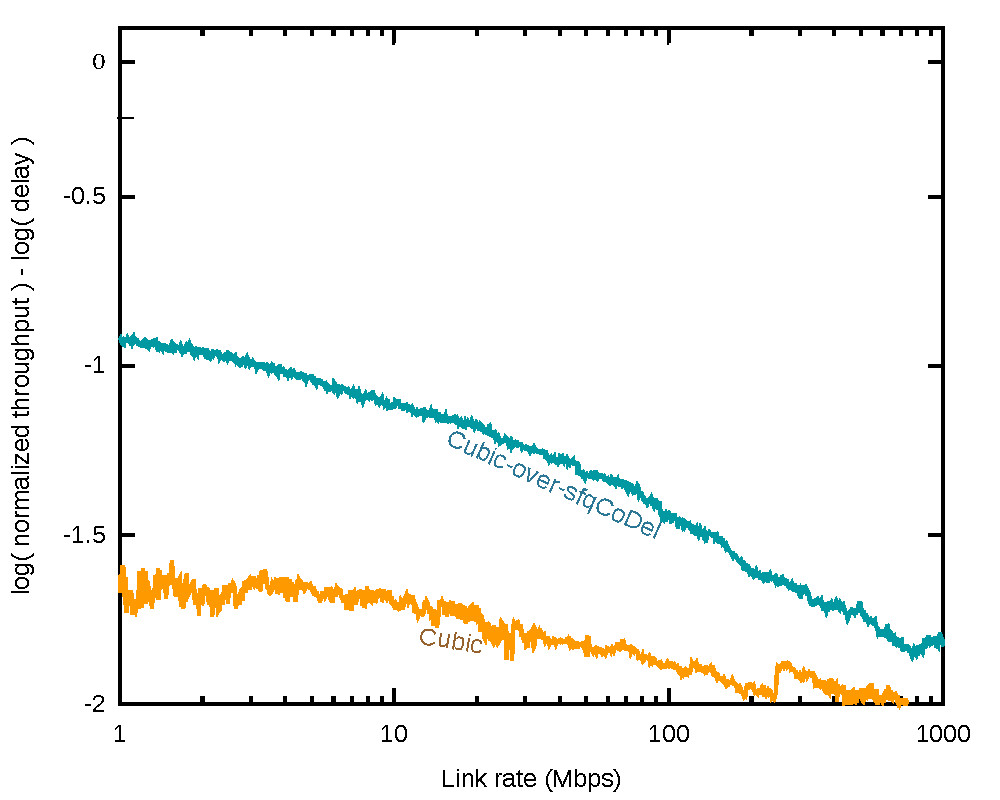
\includegraphics[width=3.1 in]{oprange-codel.pdf}}\only<4>{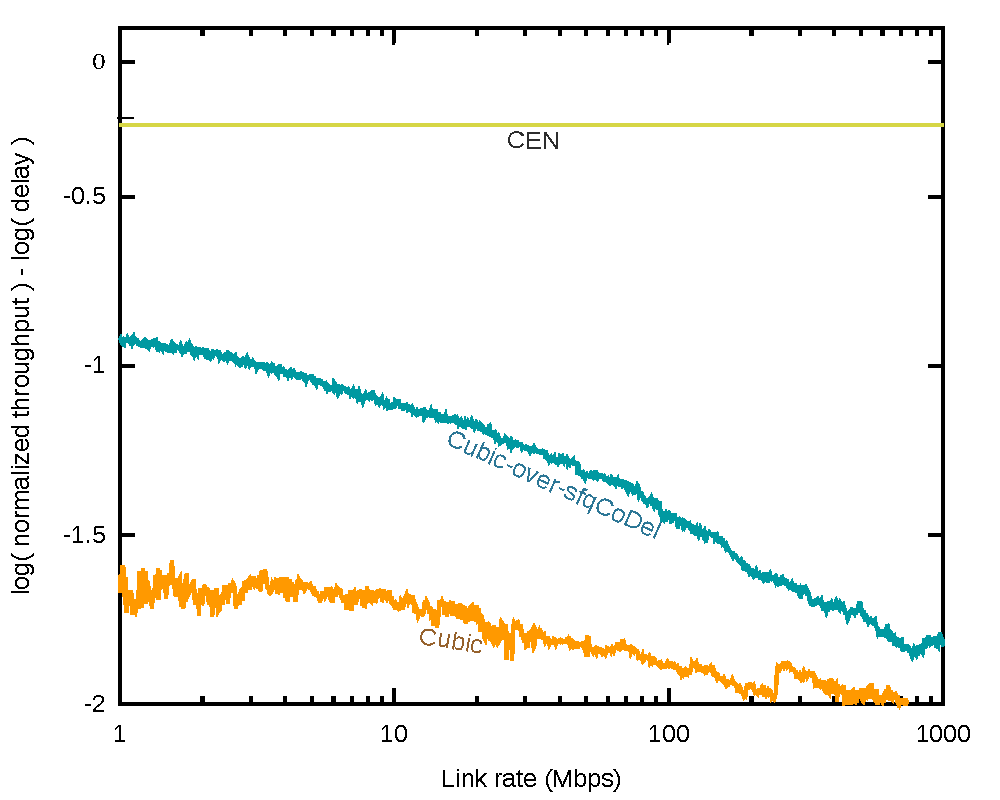
\includegraphics[width=3.1 in]{oprange-cen.pdf}}\only<5>{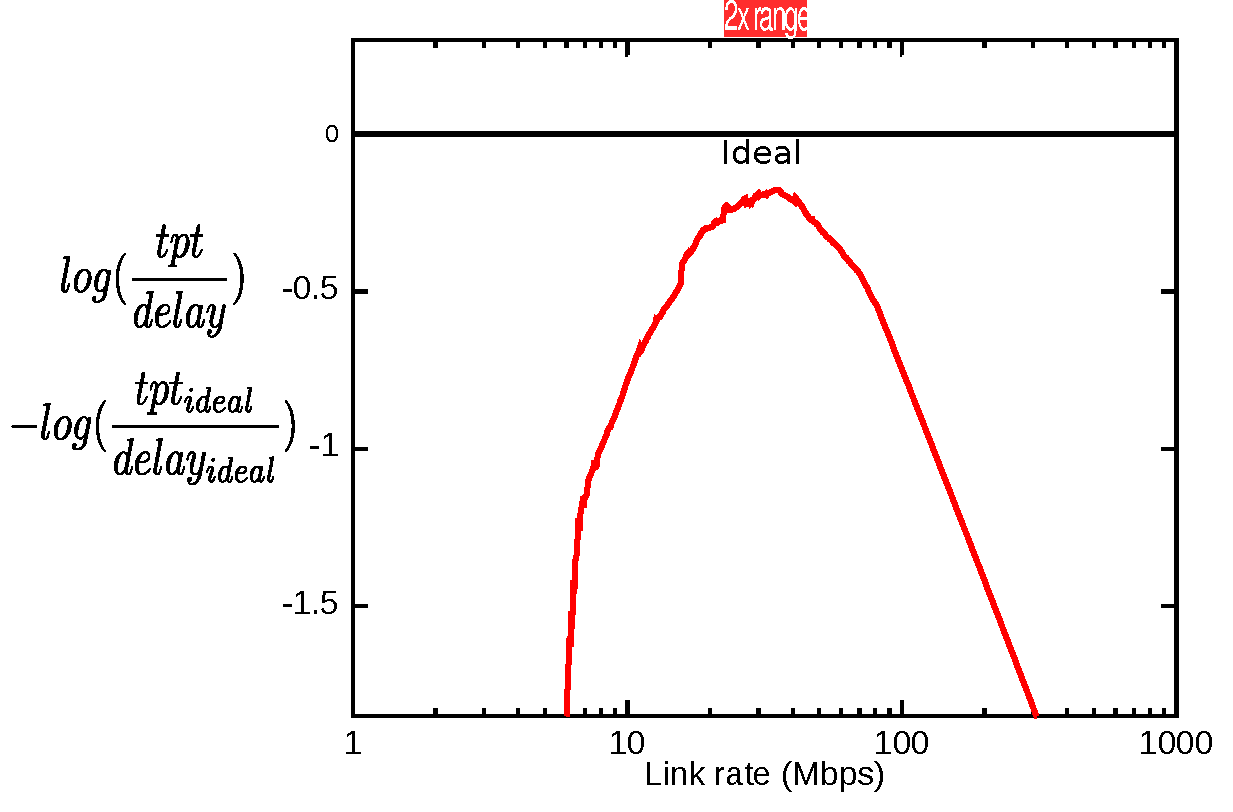
\includegraphics[width=3.1 in]{oprange-2x.pdf}}\only<6>{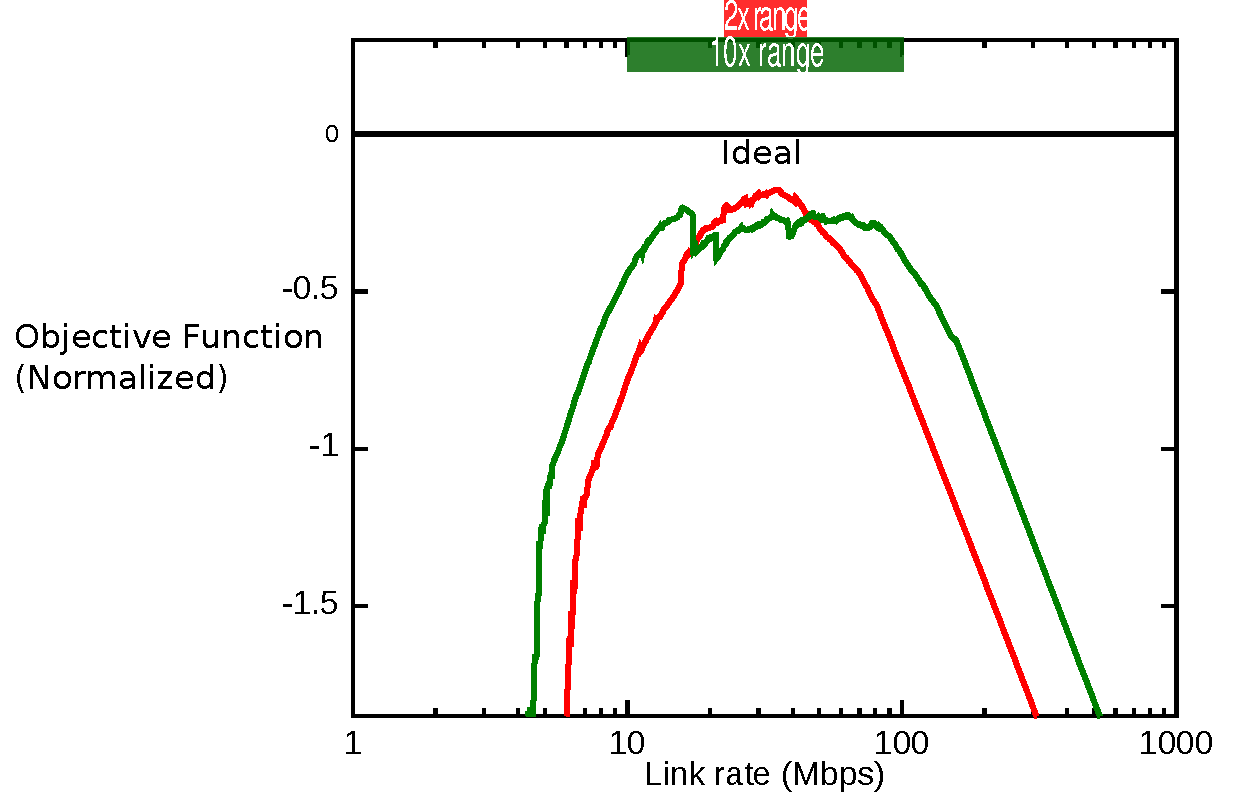
\includegraphics[width=3.1 in]{oprange-10x.pdf}}\only<7>{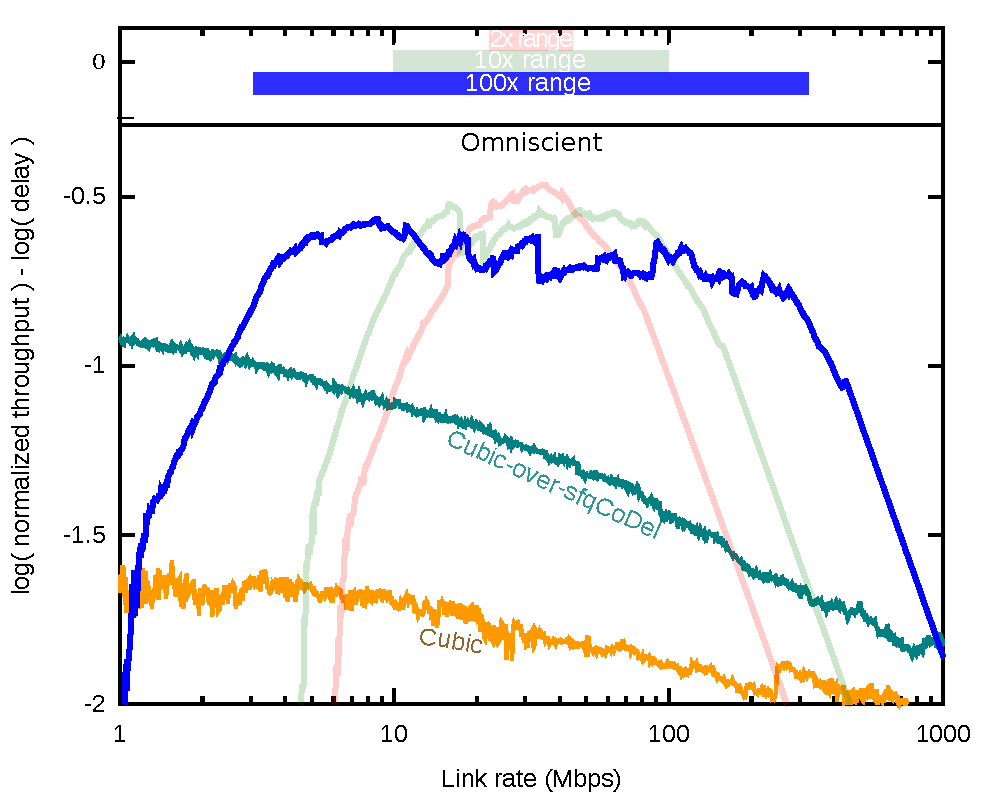
\includegraphics[width=3.1 in]{oprange-100x.pdf}}\only<8>{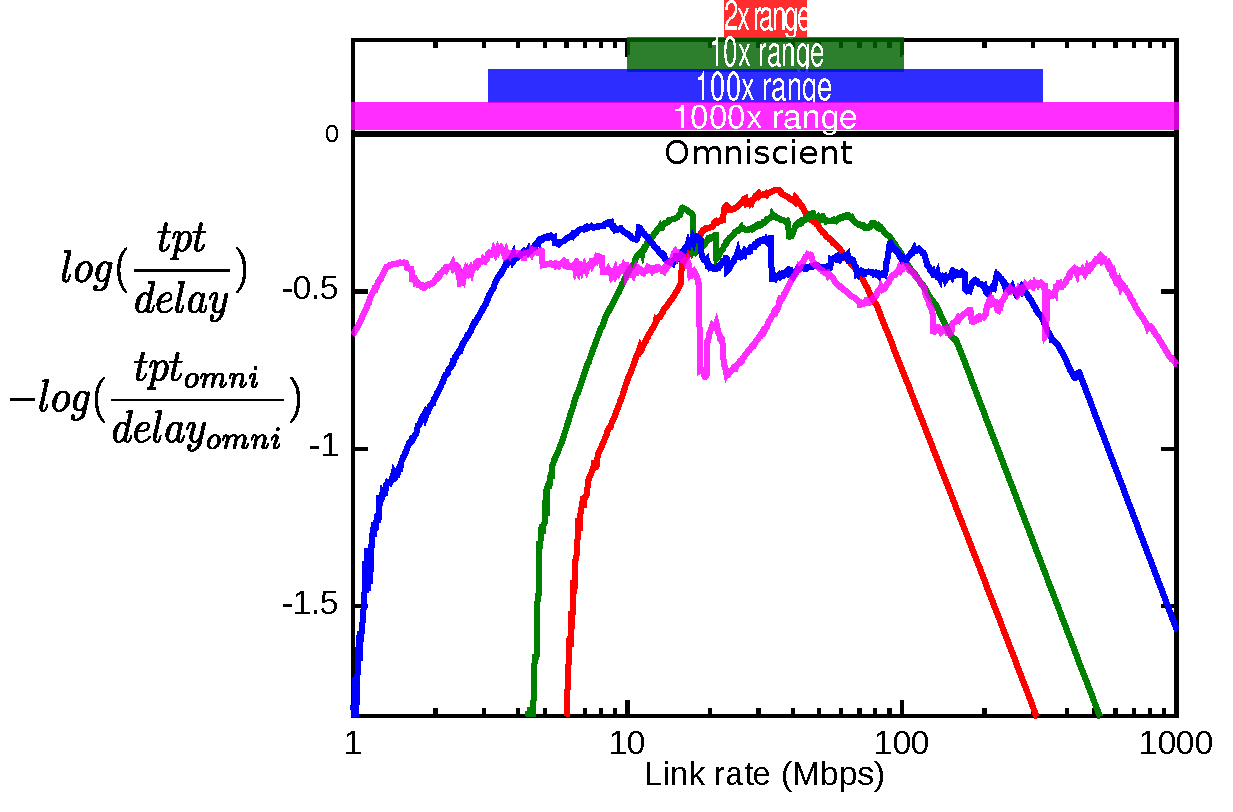
\includegraphics[width=3.1 in]{oprange-1000x.pdf}}

\end{centering}
\end{frame}
